\subsection{Reducing fixed waits in the exact reduction workflow}
The preceding comparisons show that the cost of using the seed model
depends on the full reduction workflow. Inspection of the Kira version
used here found a fixed one-second wait each time the program closed
a Fermat process. Fermat performs exact rational-function arithmetic,
and this wait occurs after the interface sends its exit command and
closes its pipes. The program then checks whether the child has exited
and forces termination if it is still running.

We replaced this fixed wait with repeated checks of the same child
process at two-millisecond intervals. The modified interface returns
as soon as it observes the exit and retains a one-second grace period
before forced termination. It also handles interrupted checks and
already reaped children. Tests checked that the arithmetic process exits normally or reaches
the existing termination limit. We built this change separately from the original
Kira executable. The symbolic elimination code, rational coefficients,
model weights and seed threshold remain unchanged
\cite{KiraResponsiveExitData}.

This change acts on a distinct part of the complete cost,
\begin{equation}
 T_{\rm total}=T_{\rm input}+T_{\rm model}+T_{\rm algebra}
             +T_{\rm exit}+T_{\rm check}.
\end{equation}
Here $T_{\rm input}$ includes loading and equation preparation,
$T_{\rm model}$ includes loading the seed model and computing its scores,
$T_{\rm algebra}$ is the time spent in exact reduction,
$T_{\rm exit}$ is the time needed to close its arithmetic processes,
and $T_{\rm check}$ is the final coefficient-verification time.
Failed attempts and fallback contribute to the corresponding terms.
Removing the fixed part of $T_{\rm exit}$ can improve a short reduction
without changing its algebraic operation count.

\subsubsection{Separating shutdown costs from learned seed selection}
We compare four complete workflows: the original Kira with all supplied
equations, the original Kira with learned seeds, the modified Kira with
all supplied equations, and the modified Kira with learned seeds.
The learned workflows use the existing model, the fixed threshold
$0.01$, the early master check and the same full-pool fallback.
Thus, comparing the two learned workflows isolates the shutdown change,
while comparing learned selection with the full pool within the modified
Kira measures the remaining benefit of that seed-selection workflow.

Development uses three instances from the original training partition.
The reserved comparison uses twelve other one-loop box instances in
six original-test kinematic groups that were absent from all earlier
box cost-test groups. Each instance has batches of one and sixteen
constructed targets, and each workflow receives five rotated repetitions
on the same node for that instance and batch size. We fixed the cases
before timing the change and froze the executable, code, model and
scientific inputs before the reserved runs.

Every measured time includes a fresh process start, input preparation,
model inference where applicable, exact Kira reduction, failed attempts,
fallback and exact coefficient checks. The prior generation of the shared
IBP identity pools is outside all four methods. Each trial uses one thread,
a 180-second complete-process cap, a 1.7 GB process-tree memory limit and
32 MiB of temporary storage. The array began with two simultaneous trials and increased to three
and then six after memory and storage checks. The individual limits,
targets, models and calculation code stayed fixed.
After a failed measured attempt, further identical repetitions are
marked as skipped and receive no measured time.

The timing comparison uses the median of five successful repetitions
for each method and batch. We form the geometric mean of their paired
time ratios and obtain descriptive 95\% intervals by resampling entire
kinematic groups 10,000 times. These intervals describe the completed
subset, and the separate completion counts retain every planned case.

Development produced 10 exact completions from 12 measured trials. The reserved comparison contains 480 planned records, 416 measured trials and 400 exact completions. Independent checks compared 8,850 sampled master-coefficient vectors with the raw Kira exports. Every completed reduction matched its exact reference coefficients.

Each workflow completed 100 trials exactly and recorded 4 failed attempts and 16 skipped repetitions. Each learned workflow used full-pool fallback 10 times among its completed trials. The paired comparisons below identify the successful batch sets.

\subsubsection{Measured complete-time changes}
For one target at a time, the modified learned workflow has a complete-time ratio of 0.385, with a descriptive 95\% interval $[0.342,0.453]$ from 12 complete paired batches relative to the original learned workflow. The corresponding geometric mean times are 5.528 and 2.126 seconds, a 61.5\% reduction. For sixteen targets, the ratio to the original learned workflow is 0.686, with a descriptive 95\% interval $[0.540,0.844]$ from 8 complete paired batches.

With the responsive shutdown active in both methods, learned seed selection has a one-target complete-time ratio of 0.690, with a descriptive 95\% interval $[0.424,0.931]$ from 11 complete paired batches relative to the full pool. The corresponding sixteen-target ratio is 0.983, with a descriptive 95\% interval $[0.915,1.063]$ from 8 complete paired batches. The one-target comparison therefore retains a measured 31.0\% reduction from the learned seed workflow after the shutdown improvement. The sixteen-target interval includes one, so a consistent additional benefit remains unresolved for that batch size.

The modified learned workflow has a one-target complete-time ratio of 0.282, with a descriptive 95\% interval $[0.199,0.349]$ from 11 complete paired batches relative to the original full-pool workflow. The full-pool workflow alone has a modified-to-original ratio of 0.408, with a descriptive 95\% interval $[0.355,0.476]$ from 11 complete paired batches. These controls show that the shutdown improvement applies to the exact solver independently of machine learning. The unchanged seed model supplies a separate choice of equations, whose incremental effect is measured against the modified full-pool control.

Across 200 completed original/modified pairs, equation inputs and reported elimination counters agreed. The final raw coefficient exports were identical in 200 pairs, and 104 paired prediction records agreed exactly. The change therefore improves process completion time while preserving the tested mathematical calculations. It does not establish fewer algebraic operations, a better trained model or a general multiloop speedup. The measured domain remains the specified supplied-identity reductions of constructed one-loop targets.

% responsive-exit-cohorts
The two learned workflows both completed all five repetitions in 12 of the twelve single-target batches and 8 of the twelve sixteen-target batches. Their successful batch sets agreed at each batch size. With the modified shutdown, learned selection alone completed 1 batch of 1 target. With the modified shutdown, the full pool alone completed 1 batch of 16 targets. The quoted ratios use only the stated complete paired subsets; all other outcomes remain in the completion counts.

% responsive-exit-cohorts-end

\begin{figure}[htbp]
\centering
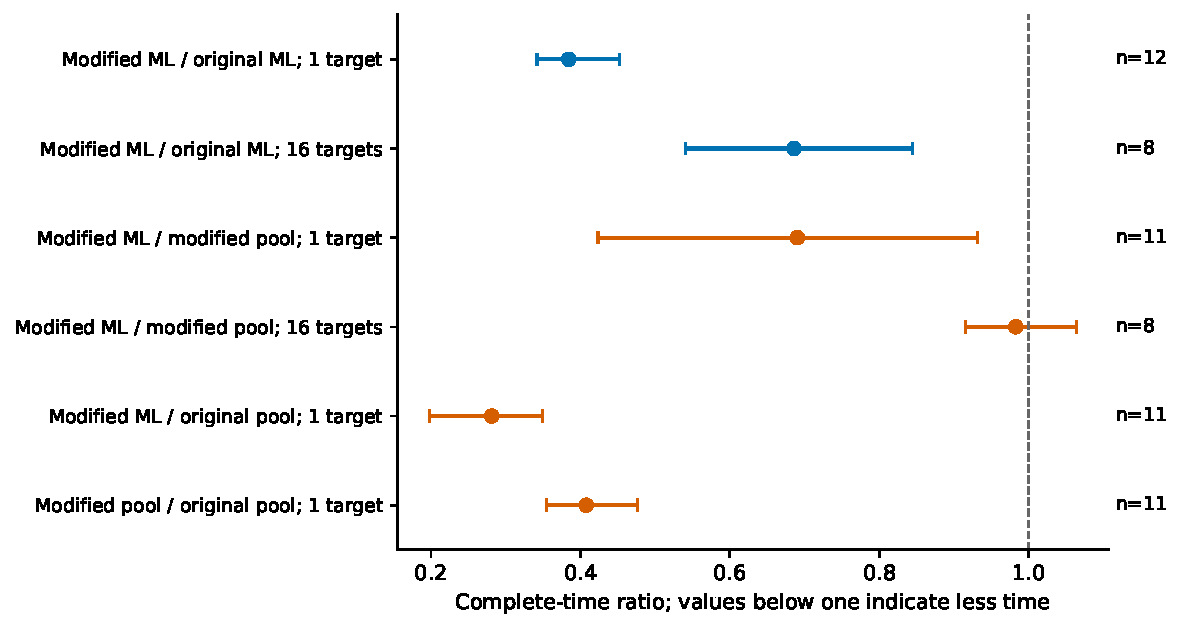
\includegraphics[width=\linewidth]{figures/responsive_exit_times.pdf}
\caption{Complete-time ratios for responsive Fermat shutdown and learned
seed selection. Points show geometric means of paired five-repeat
medians; intervals resample kinematic groups. Each row compares the
same physical targets, and values below one indicate less complete time. Here $n$ is the number of complete paired batches.}
\label{fig:responsive-exit-times}
\end{figure}
\FloatBarrier
